\begin{frame}{Rail-Editor: Übersicht}

	Übersicht:
	\begin{itemize}
		\item Softwaretechnik
		\item Technische Aspekte
		\item Live-Demo
	\end{itemize}

\end{frame}

\pagebreak

\begin{frame}{Rail-Editor: Softwaretechnik}
	\begin{itemize}
		\item kleines Team $\rightarrow$ Kommunikation per Email
		\pause
		\item direkte Reaktionen auf Emails (an alle geschickt)
		\pause
		\item zuerst zwei, nach dem ersten Milestone drei Mitglieder
		\begin{itemize}
			\item bessere Arbeitsverteilung
		\end{itemize}
		\pause
		\item Teilnahme an Daily Scrums (montags und mittwochs)
		\pause
		\item zusätzliche Team-Meetings außer donnerstags
		\begin{itemize}
			\item produktives Arbeiten durch Pair-Programming
		\end{itemize}
		\pause
		\item gute Kommunikation innerhalb des Teams
		\pause
		\item anfangs spärliche Kommunikation mit anderen Teams
	\end{itemize}
\end{frame}

\begin{frame}{Rail-Editor: Technische Aspekte I}
	\begin{itemize}
		\item \textit{QT} für Programmierung der grafischen Benutzeroberfläche
		\pause
		\item Signal- und Slottechnik
		\pause
		\item Eventverarbeitung für Maus- und Tastendrücke
		\pause
		\item Basisklassen abgeleitet und Funktionalitäten erweitert
		\pause
		\item Graphstruktur für Syntax-Highlighting
		\begin{itemize}
			\item internes Backend
		\end{itemize}
		\pause
		\item Smart-Cursor und Grab-Modus
		\begin{itemize}
			\item für intuitives Schreiben von Quellcode
			\item siehe Live-Demo
		\end{itemize}
	\end{itemize}
\end{frame}

\begin{frame}{Rail-Editor: Technische Aspekte II}
	\begin{itemize}
		\item Main-Window als \textit{Brain}
		\begin{itemize}
			\item Weiterleitung an Child-Widgets
		\end{itemize}
		\pause
		\item Undo-Redo-Funktionalität
		\begin{itemize}
			\item abstrakte Klasse
			\item wird durch konkrete Aktionen implementiert
		\end{itemize}
		\pause
		\item Compiler-Einbindung
		\begin{itemize}
			\item Funktionen: Build, Run, Stop
			\item auch der Rail-Interpreter kann verwendet werden
		\end{itemize}
		\pause
		\item \textit{Preferences} (Editor-Einstellungen)
		\begin{itemize}
			\item persistent gespeichert
		\end{itemize}
	\end{itemize}
	\pause
	
	\begin{figure}
		\centering
		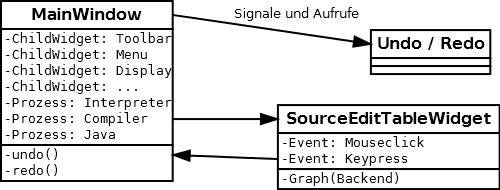
\includegraphics[width=0.7\textwidth]{editor-uebersicht}
	\end{figure}
\end{frame}
